\documentclass[11pt]{article}

\usepackage[margin=1in]{geometry}
\usepackage{amsmath}
\usepackage{booktabs}
\usepackage{graphicx}
\usepackage{float}
\usepackage{siunitx}

\title{Numerical Stability of Explicit and Implicit Methods for a Bounded Memristor ODE}
\author{John Louis Lagramada \and Patrick Villareal}
\date{}

\begin{document}

\maketitle

\section{Overview}

This project studies the numerical behavior of three single-step methods applied to a nonlinear memristor initial value problem. The objective is not only to compute a trajectory, but to compare how each method reacts when the time step becomes coarse relative to the time scale of the excitation. The main quantities of interest are the internal state trajectory, violations of the physical state bounds, and the resulting voltage-current hysteresis loops.

\section{Memristor Model}

The device is modeled using the linear ion drift HP TiO2 memristor model. The internal state variable \(w(t)\) represents the width of the doped region. It is physically constrained by
\[
0 \leq w(t) \leq D,
\]
where \(D\) is the device thickness.

The memristance is
\[
M(w) = R_{\text{on}}\frac{w}{D}
       + R_{\text{off}}\left(1-\frac{w}{D}\right),
\]
with applied voltage
\[
v(t) = V_0 \sin(\omega t).
\]
The current is then
\[
i(t,w) = \frac{v(t)}{M(w)}.
\]
The state equation solved numerically is
\[
\frac{dw}{dt}
=
\frac{\mu_v R_{\text{on}} v(t)}{D^2 M(w)}.
\]

\section{Numerical Methods}

The initial value problem was solved using Explicit Euler, fourth-order Runge-Kutta, and Implicit Euler. Explicit Euler advances the state using the derivative at the current time. RK4 uses four slope evaluations per step to obtain a higher-order explicit approximation. Implicit Euler advances the state using the derivative at the next time, which requires solving a nonlinear scalar equation at every step.

For Implicit Euler, the update satisfies
\[
w_{n+1} = w_n + h f(t_{n+1}, w_{n+1}),
\]
or equivalently
\[
F(w_{n+1}) = w_{n+1} - w_n - h f(t_{n+1}, w_{n+1}) = 0.
\]
This scalar nonlinear equation is solved by Newton iteration using an Explicit Euler prediction as the initial guess.

\section{Experiment Design}

The notebook evaluates all methods over the same time interval and with the same initial condition. Several step sizes are used, ranging from fine to deliberately coarse. Raw trajectories are preserved so that unphysical overshoot can be measured directly. A clipped copy of each trajectory is also computed for voltage-current plots, because the physical memristor interpretation requires \(w\) to remain in \([0,D]\).

The comparison uses four output types:

\begin{itemize}
  \item state trajectory plots \(w(t)/D\),
  \item overshoot summaries measuring how far raw states leave the interval \([0,D]\),
  \item V-I hysteresis loops computed from clipped states,
  \item runtime summaries measuring median cost per step over repeated solver calls.
\end{itemize}

\section{Results}

Figure~\ref{fig:state} compares the raw state trajectories. The step labels should be read carefully: \(T/400\) is the finest step size, while \(T/8\) is the coarsest. The plot should not be interpreted as a monotone ranking where coarser steps always create larger overshoot. In this stress test, the raw mathematical update is not bound-preserving, and coarse time steps can also miss parts of the sinusoidal forcing. Therefore, a coarse trajectory that stays inside \([0,D]\) is not automatically more accurate; it may simply be under-resolving the dynamics.

\begin{figure}[H]
  \centering
  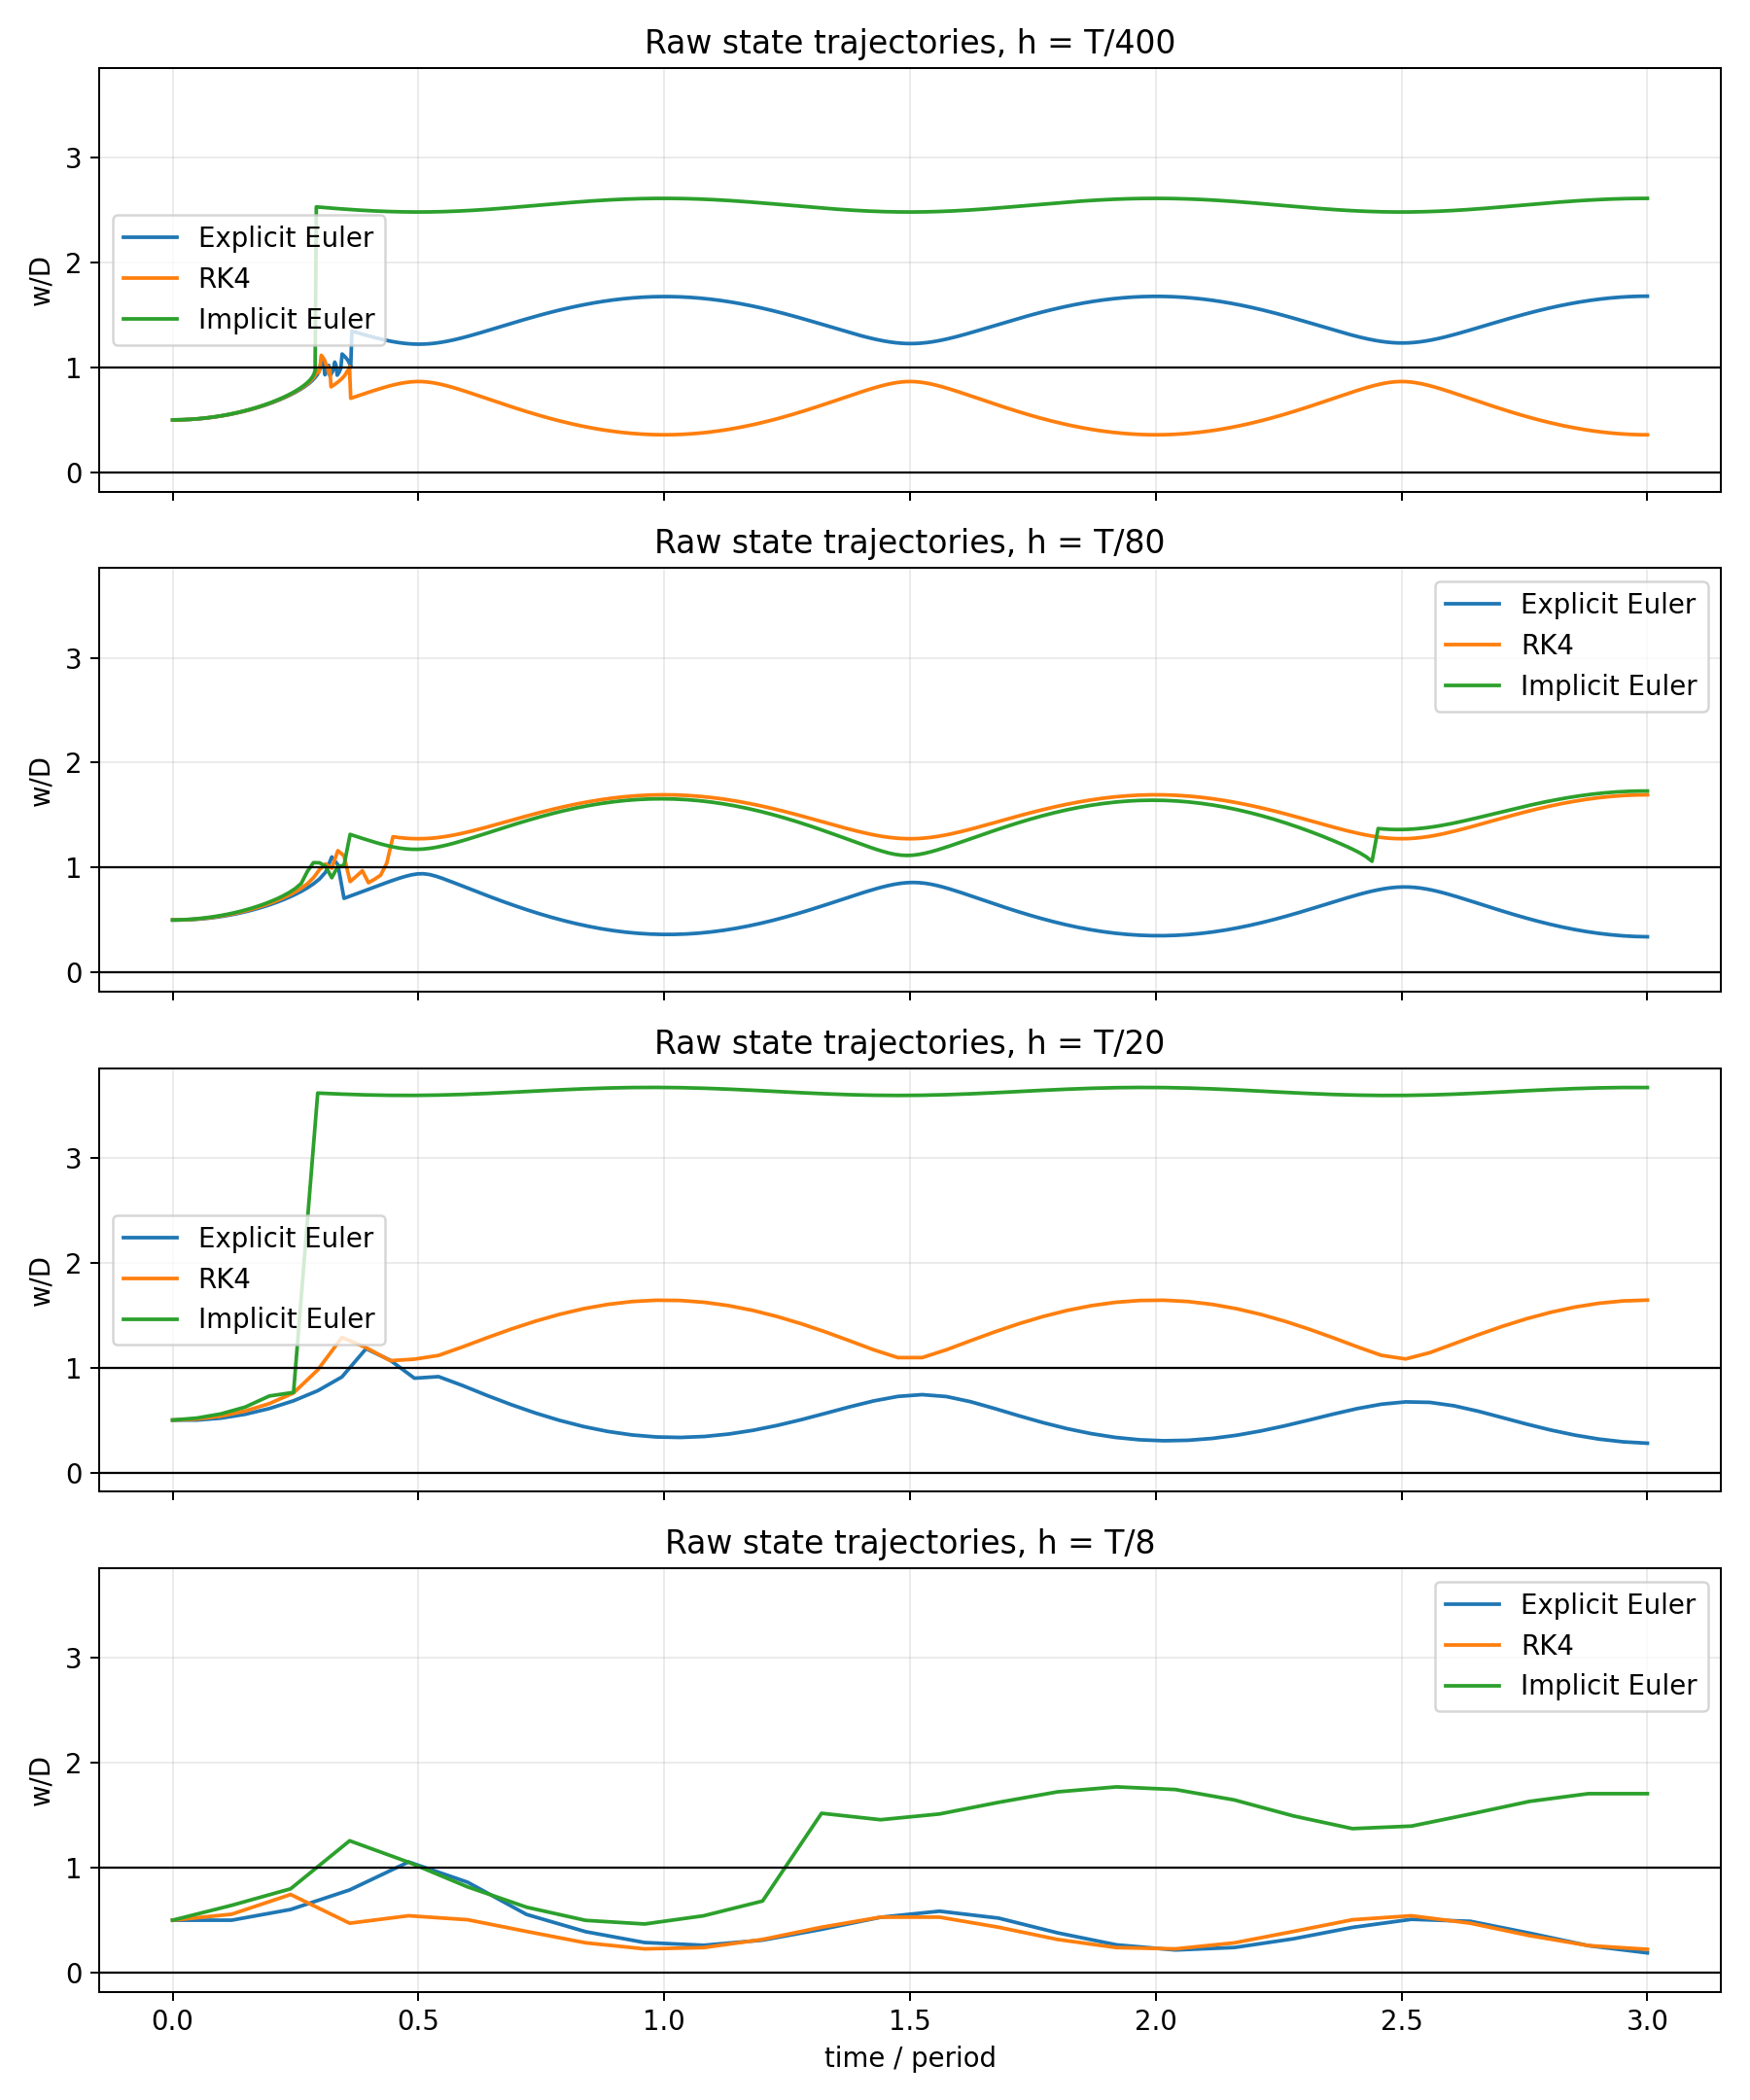
\includegraphics[width=\linewidth]{../figures/state_trajectories.png}
  \caption{Raw normalized state trajectories for the tested methods and step sizes.}
  \label{fig:state}
\end{figure}

Figure~\ref{fig:bounds} summarizes boundary violations. This view makes the physical constraint explicit and helps distinguish a numerically smooth trajectory from one that is physically meaningful. A small bar should be read together with the state plot: it can mean the method preserved the bounds, but it can also mean the method skipped over important dynamics because the step size was too coarse.

\begin{figure}[H]
  \centering
  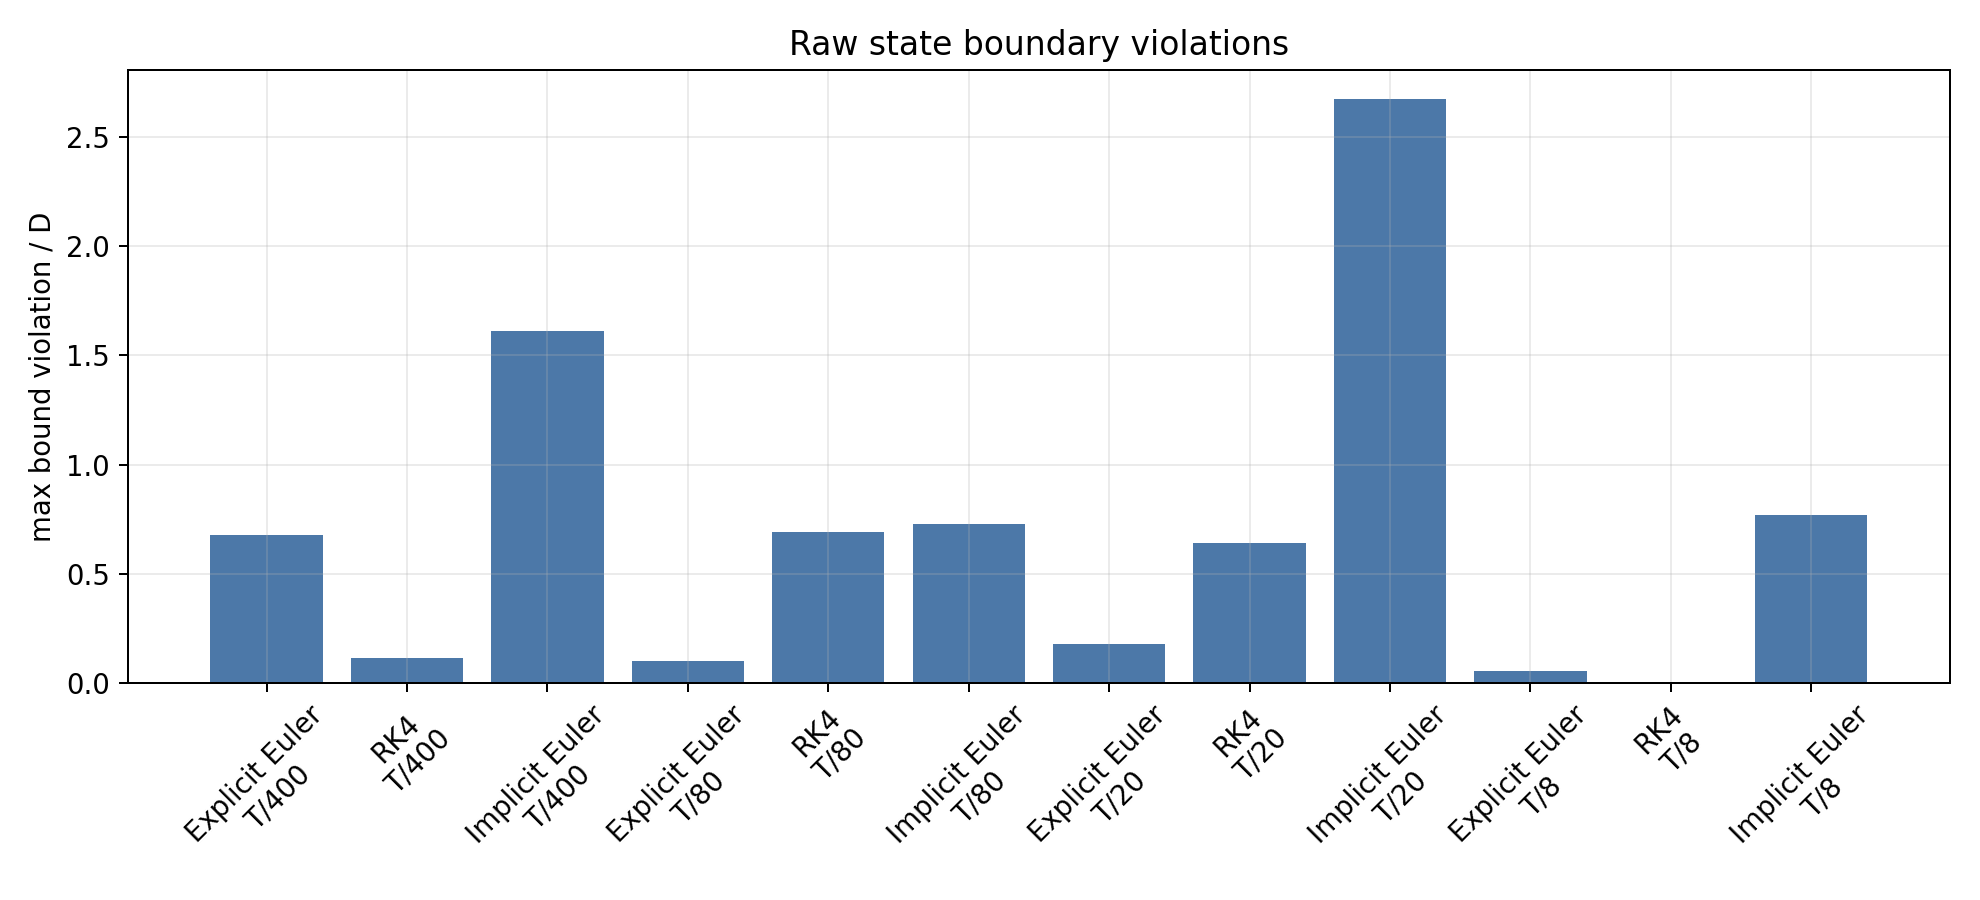
\includegraphics[width=\linewidth]{../figures/bound_violations.png}
  \caption{Raw state bounds compared against the physical interval \(0 \leq w \leq D\).}
  \label{fig:bounds}
\end{figure}

Figure~\ref{fig:hysteresis} shows the resulting voltage-current curves using clipped physical states. Clipping is used only for this physical visualization; the overshoot tables are computed from raw trajectories.

\begin{figure}[H]
  \centering
  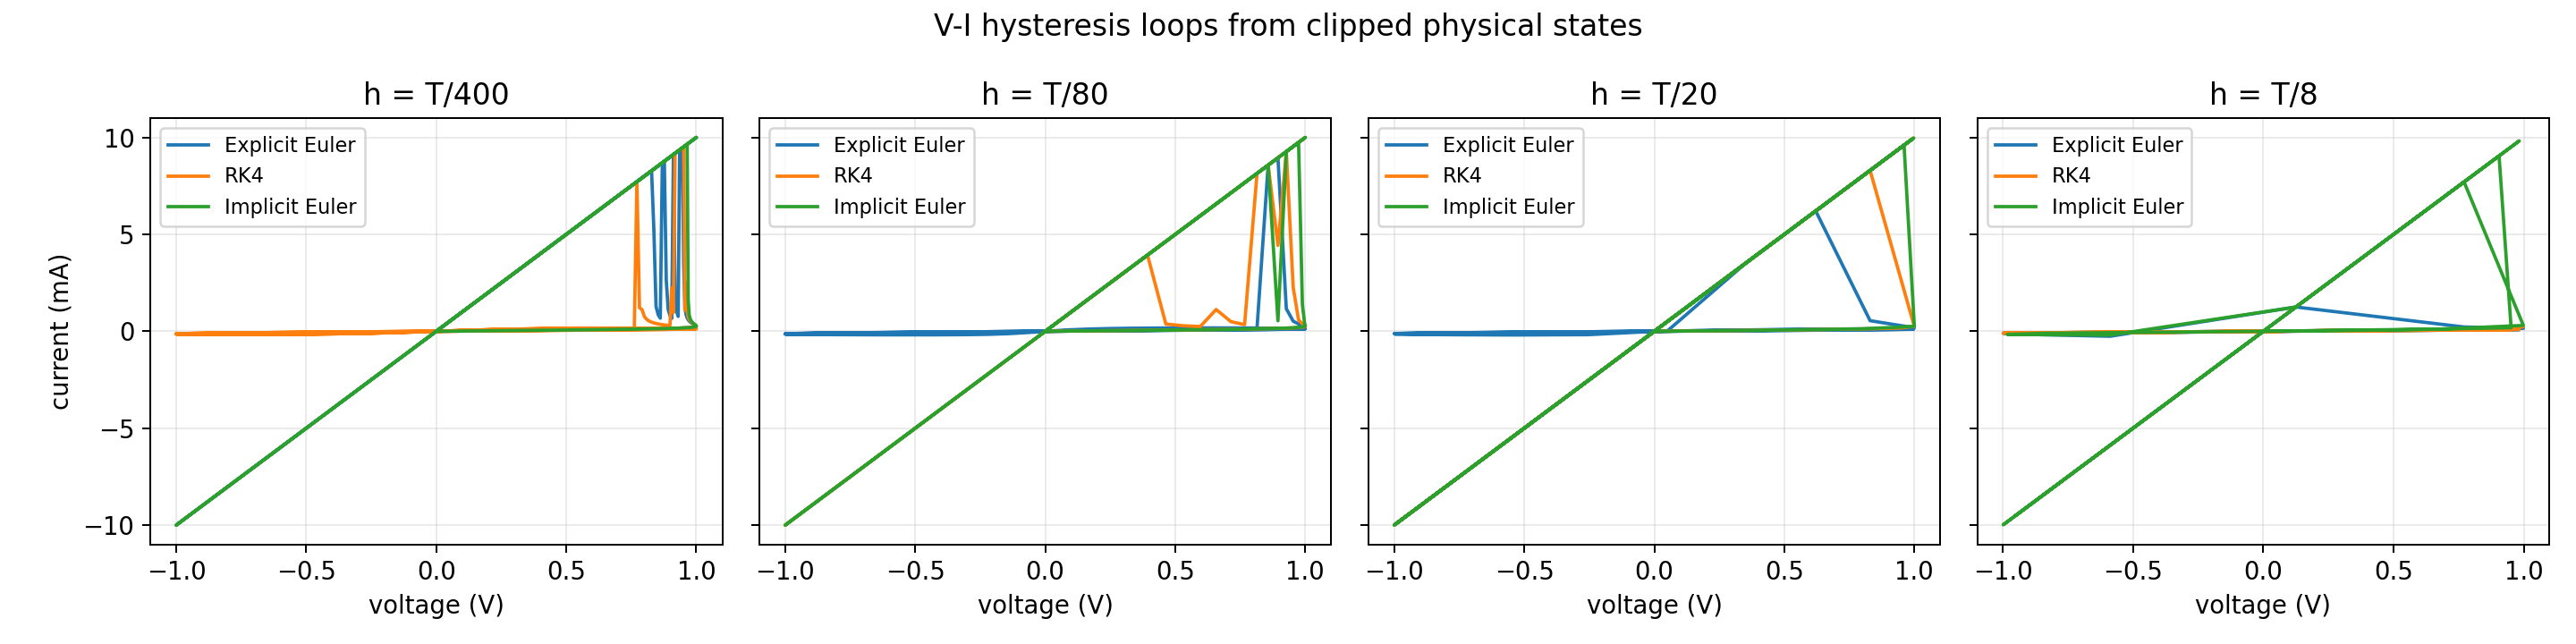
\includegraphics[width=\linewidth]{../figures/hysteresis_loops.png}
  \caption{Voltage-current hysteresis loops computed from clipped physical states.}
  \label{fig:hysteresis}
\end{figure}

Figure~\ref{fig:runtime} reports relative runtime per step. These timings are not hardware-independent benchmarks, but they show the expected computational-cost pattern: Explicit Euler is cheapest per step, RK4 pays for four slope evaluations, and Implicit Euler pays for nonlinear solves. Runtime alone does not determine the best method. A cheap method that gives an under-resolved or unphysical trajectory is not better simply because it runs faster.

\begin{figure}[H]
  \centering
  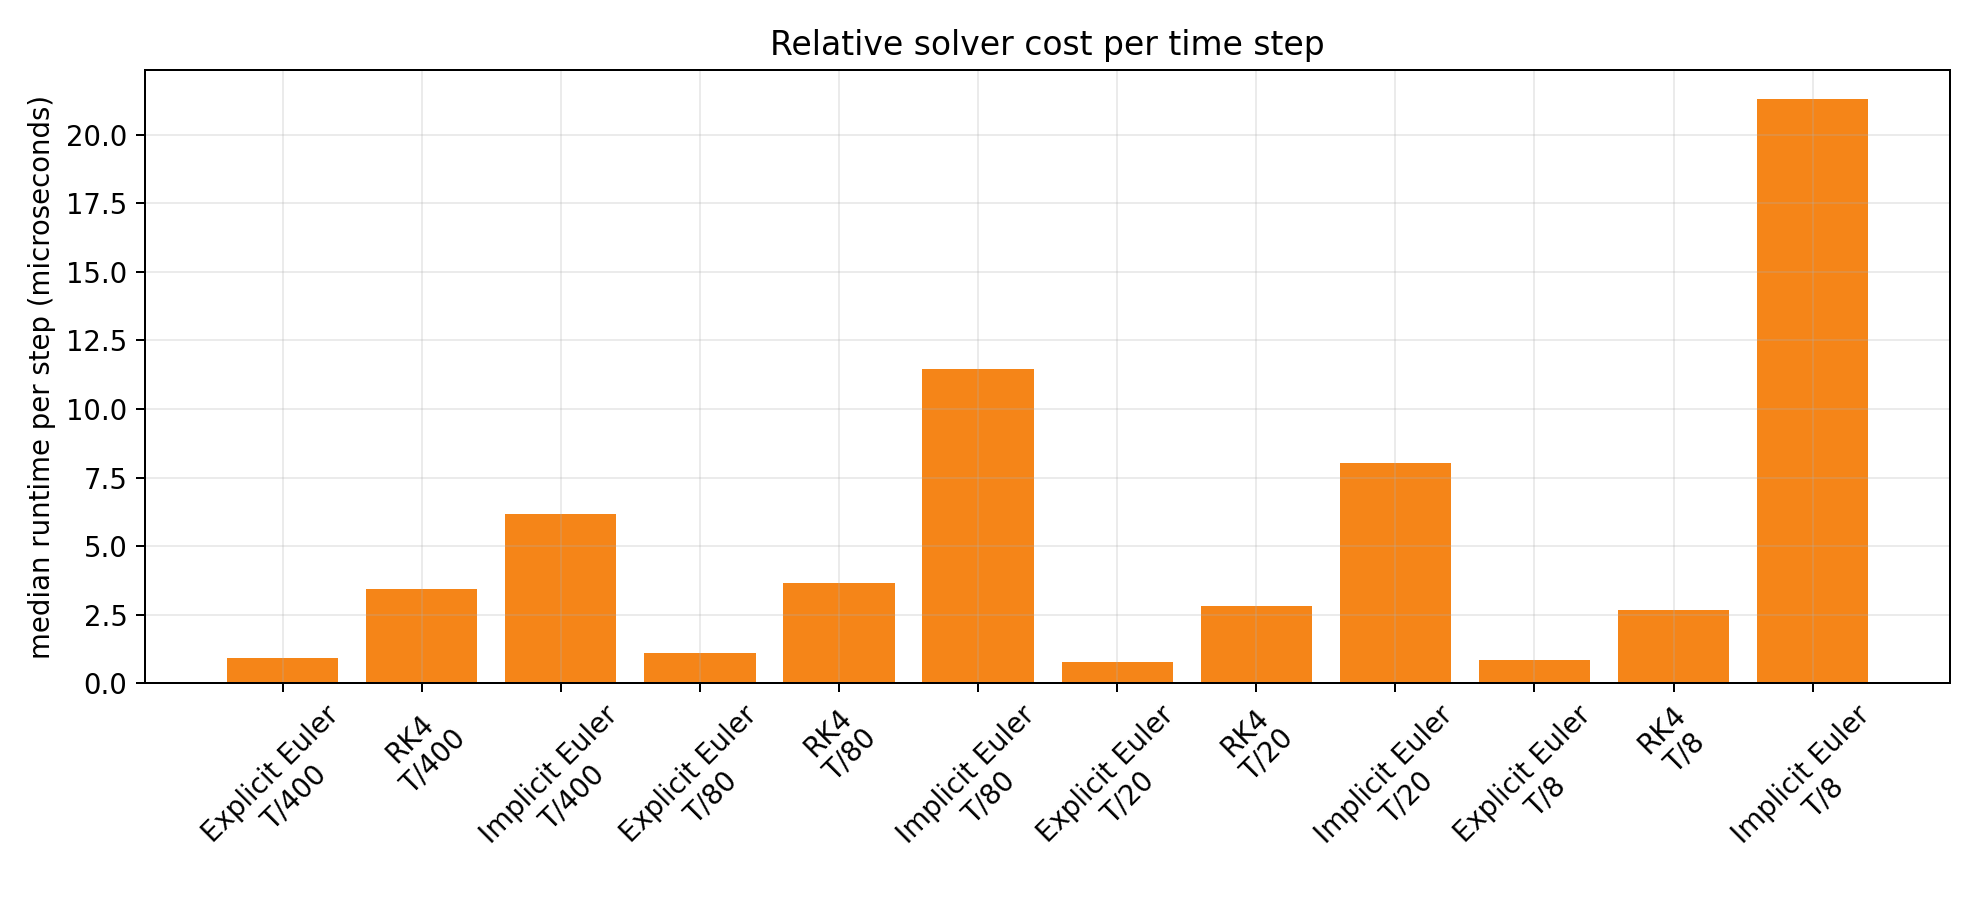
\includegraphics[width=\linewidth]{../figures/runtime_per_step.png}
  \caption{Median runtime per step over repeated solver calls.}
  \label{fig:runtime}
\end{figure}

\section{Discussion}

The project illustrates the tradeoff between accuracy, stability, and computational cost. Explicit Euler is simple but strongly step-size dependent. RK4 is more accurate for smooth trajectories at a given step size, but it is still explicit and can exhibit unphysical behavior when the step size is too coarse. Implicit Euler is only first-order accurate, and its future-time derivative can improve damping for stable modes, but it does not automatically enforce the memristor bounds. In this bounded nonlinear model, raw implicit updates can still leave the physical interval unless bound handling is added separately.

For this memristor problem, physical interpretation matters as much as numerical smoothness. A method can produce a curve that appears computationally well behaved while still violating \(0 \leq w \leq D\). Preserving raw trajectories and separately clipping them for physical current calculations makes this distinction visible.

The non-monotone behavior across step sizes is an important presentation point. For example, RK4 can look reasonable at \(T/400\), overshoot for \(T/80\) or \(T/20\), and then appear bounded again at \(T/8\). This does not mean the coarsest RK4 run is best. It means the coarse grid is sampling the forcing so sparsely that it can miss the state movement that causes overshoot. Likewise, Explicit Euler can look attractive because it is cheap and may show smaller overshoot in some cases, but that does not prove it is the most accurate method. It is still first-order and can be wrong for reasons that are not visible from the boundary bar alone.

Another reason the raw plots are irregular is the form of the memristance. With the default parameters, the linear expression for \(M(w)\) approaches zero shortly above the physical upper bound. Once a raw trajectory crosses beyond \(D\), the denominator in \(dw/dt\) can become very small, so small numerical differences can cause large changes in the next update. This makes the raw plot a stress test of the unconstrained numerical methods, not a clean proof that one method dominates all others.

\section{Conclusion}

Explicit Euler, RK4, and Implicit Euler provide different views of the bounded memristor IVP. RK4 is generally the most reliable explicit accuracy baseline when the step size is sufficiently small and the trajectory is resolved. Explicit Euler is cheapest, but cheapness does not compensate for first-order accuracy and possible under-resolution. Implicit Euler requires nonlinear solves and may improve stability for some dynamics, but it is not a substitute for physical state constraints. The results support the proposal's central point: step-size choice, method behavior, and boundary treatment strongly affect whether the simulated memristor remains physically meaningful.

\end{document}
